% Figure 2: learner actions per soup step, all personas and both algorithms in one plot.
% colour = persona; P (left) = PPO, G (right) = GRPO; o = next to greedy, x = alone (greedy frozen);
% orange o at the centre of each step = the greedy partner's own actions next to the learners (mean over
%   personas, algorithms and seeds);
% orange x at the centre of each step = greedy alone (learner frozen), mean over the PPO and GRPO configs.
% y axis: linear 0-5, log above. Step 4 (wait) is not an action: grey band, no data.
% GENERATED by eval/fig_steps.py from results/train/overcooked/fig_steps.csv and results/train/overcooked/fig_steps_greedy.csv. Do not edit by hand; rerun the script.
% Use inside a one-column figure (width = \columnwidth).
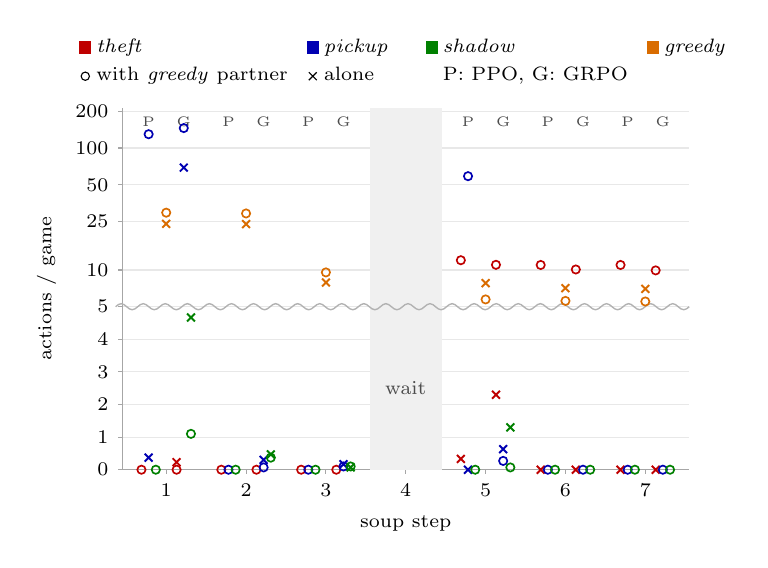
\begin{tikzpicture}
\begin{axis}[
  scale only axis, width=7.2cm, height=4.6cm, font=\scriptsize,
  xmin=0.45, xmax=7.55, xtick={1,...,7}, xlabel={soup step},
  y coord trafo/.code={\pgfmathparse{(#1<=5.0) ? (0.45*#1/5.0) : (0.45+0.55*ln(max(#1,5.0)/5.0)/ln(43.0))}},
  y coord inv trafo/.code={\pgfmathparse{#1}},
  ymin=0, ymax=215, ytick={0,1,2,3,4,5,10,25,50,100,200}, yticklabels={0,1,2,3,4,5,10,25,50,100,200}, ylabel={actions / game},
  tick align=outside, xtick pos=bottom, ytick pos=left, major tick length=1.5pt,
  axis x line*=bottom, axis y line*=left, axis line style={gray!70}, every tick/.style={gray!70},
  ymajorgrids, grid style={gray!18}, clip=false,
  legend style={font=\scriptsize, draw=none, fill=none, at={(0.5,1.03)}, anchor=south, legend columns=4,
                cells={anchor=west}, /tikz/every even column/.append style={column sep=5pt}},
]
\fill[gray!12] (axis cs:3.55,0) rectangle (axis cs:4.45,215);
\node[gray!60!black] at (axis cs:4,2.5) {wait};
\draw[gray!60, line width=0.5pt] ([xshift=-2.4pt]axis cs:0.45,5) sin ++(1.993pt,1.1pt) cos ++(1.993pt,-1.1pt) sin ++(1.993pt,-1.1pt) cos ++(1.993pt,1.1pt) sin ++(1.993pt,1.1pt) cos ++(1.993pt,-1.1pt) sin ++(1.993pt,-1.1pt) cos ++(1.993pt,1.1pt) sin ++(1.993pt,1.1pt) cos ++(1.993pt,-1.1pt) sin ++(1.993pt,-1.1pt) cos ++(1.993pt,1.1pt) sin ++(1.993pt,1.1pt) cos ++(1.993pt,-1.1pt) sin ++(1.993pt,-1.1pt) cos ++(1.993pt,1.1pt) sin ++(1.993pt,1.1pt) cos ++(1.993pt,-1.1pt) sin ++(1.993pt,-1.1pt) cos ++(1.993pt,1.1pt) sin ++(1.993pt,1.1pt) cos ++(1.993pt,-1.1pt) sin ++(1.993pt,-1.1pt) cos ++(1.993pt,1.1pt) sin ++(1.993pt,1.1pt) cos ++(1.993pt,-1.1pt) sin ++(1.993pt,-1.1pt) cos ++(1.993pt,1.1pt) sin ++(1.993pt,1.1pt) cos ++(1.993pt,-1.1pt) sin ++(1.993pt,-1.1pt) cos ++(1.993pt,1.1pt) sin ++(1.993pt,1.1pt) cos ++(1.993pt,-1.1pt) sin ++(1.993pt,-1.1pt) cos ++(1.993pt,1.1pt) sin ++(1.993pt,1.1pt) cos ++(1.993pt,-1.1pt) sin ++(1.993pt,-1.1pt) cos ++(1.993pt,1.1pt) sin ++(1.993pt,1.1pt) cos ++(1.993pt,-1.1pt) sin ++(1.993pt,-1.1pt) cos ++(1.993pt,1.1pt) sin ++(1.993pt,1.1pt) cos ++(1.993pt,-1.1pt) sin ++(1.993pt,-1.1pt) cos ++(1.993pt,1.1pt) sin ++(1.993pt,1.1pt) cos ++(1.993pt,-1.1pt) sin ++(1.993pt,-1.1pt) cos ++(1.993pt,1.1pt) sin ++(1.993pt,1.1pt) cos ++(1.993pt,-1.1pt) sin ++(1.993pt,-1.1pt) cos ++(1.993pt,1.1pt) sin ++(1.993pt,1.1pt) cos ++(1.993pt,-1.1pt) sin ++(1.993pt,-1.1pt) cos ++(1.993pt,1.1pt) sin ++(1.993pt,1.1pt) cos ++(1.993pt,-1.1pt) sin ++(1.993pt,-1.1pt) cos ++(1.993pt,1.1pt) sin ++(1.993pt,1.1pt) cos ++(1.993pt,-1.1pt) sin ++(1.993pt,-1.1pt) cos ++(1.993pt,1.1pt) sin ++(1.993pt,1.1pt) cos ++(1.993pt,-1.1pt) sin ++(1.993pt,-1.1pt) cos ++(1.993pt,1.1pt) sin ++(1.993pt,1.1pt) cos ++(1.993pt,-1.1pt) sin ++(1.993pt,-1.1pt) cos ++(1.993pt,1.1pt) sin ++(1.993pt,1.1pt) cos ++(1.993pt,-1.1pt) sin ++(1.993pt,-1.1pt) cos ++(1.993pt,1.1pt) sin ++(1.993pt,1.1pt) cos ++(1.993pt,-1.1pt) sin ++(1.993pt,-1.1pt) cos ++(1.993pt,1.1pt) sin ++(1.993pt,1.1pt) cos ++(1.993pt,-1.1pt) sin ++(1.993pt,-1.1pt) cos ++(1.993pt,1.1pt) sin ++(1.993pt,1.1pt) cos ++(1.993pt,-1.1pt) sin ++(1.993pt,-1.1pt) cos ++(1.993pt,1.1pt) sin ++(1.993pt,1.1pt) cos ++(1.993pt,-1.1pt) sin ++(1.993pt,-1.1pt) cos ++(1.993pt,1.1pt) sin ++(1.993pt,1.1pt) cos ++(1.993pt,-1.1pt) sin ++(1.993pt,-1.1pt) cos ++(1.993pt,1.1pt) sin ++(1.993pt,1.1pt) cos ++(1.993pt,-1.1pt) sin ++(1.993pt,-1.1pt) cos ++(1.993pt,1.1pt);
\node[gray!60!black, font=\tiny, anchor=north] at (axis cs:0.78,215) {P};
\node[gray!60!black, font=\tiny, anchor=north] at (axis cs:1.22,215) {G};
\node[gray!60!black, font=\tiny, anchor=north] at (axis cs:1.78,215) {P};
\node[gray!60!black, font=\tiny, anchor=north] at (axis cs:2.22,215) {G};
\node[gray!60!black, font=\tiny, anchor=north] at (axis cs:2.78,215) {P};
\node[gray!60!black, font=\tiny, anchor=north] at (axis cs:3.22,215) {G};
\node[gray!60!black, font=\tiny, anchor=north] at (axis cs:4.78,215) {P};
\node[gray!60!black, font=\tiny, anchor=north] at (axis cs:5.22,215) {G};
\node[gray!60!black, font=\tiny, anchor=north] at (axis cs:5.78,215) {P};
\node[gray!60!black, font=\tiny, anchor=north] at (axis cs:6.22,215) {G};
\node[gray!60!black, font=\tiny, anchor=north] at (axis cs:6.78,215) {P};
\node[gray!60!black, font=\tiny, anchor=north] at (axis cs:7.22,215) {G};
% ppo theft
\addplot[red!75!black, only marks, mark=o, mark size=1.5pt, line width=0.6pt, forget plot] coordinates {(0.69,0.00) (1.69,0.00) (2.69,0.00) (4.69,12.03) (5.69,11.00) (6.69,11.00)};
\addplot[red!75!black, only marks, mark=x, mark size=2pt, line width=0.7pt, forget plot] coordinates {(4.69,0.33) (5.69,0.00) (6.69,0.00)};
% grpo theft
\addplot[red!75!black, only marks, mark=o, mark size=1.5pt, line width=0.6pt, forget plot] coordinates {(1.13,0.00) (2.13,0.00) (3.13,0.00) (5.13,11.03) (6.13,10.10) (7.13,9.93)};
\addplot[red!75!black, only marks, mark=x, mark size=2pt, line width=0.7pt, forget plot] coordinates {(1.13,0.23) (5.13,2.30) (6.13,0.00) (7.13,0.00)};
% ppo pickup
\addplot[blue!70!black, only marks, mark=o, mark size=1.5pt, line width=0.6pt, forget plot] coordinates {(0.78,129.87) (1.78,0.00) (2.78,0.00) (4.78,58.80) (5.78,0.00) (6.78,0.00)};
\addplot[blue!70!black, only marks, mark=x, mark size=2pt, line width=0.7pt, forget plot] coordinates {(0.78,0.37) (4.78,0.00)};
% grpo pickup
\addplot[blue!70!black, only marks, mark=o, mark size=1.5pt, line width=0.6pt, forget plot] coordinates {(1.22,145.83) (2.22,0.07) (3.22,0.10) (5.22,0.27) (6.22,0.00) (7.22,0.00)};
\addplot[blue!70!black, only marks, mark=x, mark size=2pt, line width=0.7pt, forget plot] coordinates {(1.22,69.13) (2.22,0.30) (3.22,0.17) (5.22,0.63)};
% ppo shadow
\addplot[green!50!black, only marks, mark=o, mark size=1.5pt, line width=0.6pt, forget plot] coordinates {(0.87,0.00) (1.87,0.00) (2.87,0.00) (4.87,0.00) (5.87,0.00) (6.87,0.00)};
% grpo shadow
\addplot[green!50!black, only marks, mark=o, mark size=1.5pt, line width=0.6pt, forget plot] coordinates {(1.31,1.10) (2.31,0.37) (3.31,0.10) (5.31,0.07) (6.31,0.00) (7.31,0.00)};
\addplot[green!50!black, only marks, mark=x, mark size=2pt, line width=0.7pt, forget plot] coordinates {(1.31,4.67) (2.31,0.47) (3.31,0.07) (5.31,1.30)};
% greedy next to the learners (mean over personas, algorithms and seeds)
\addplot[orange!85!black, only marks, mark=o, mark size=1.5pt, line width=0.6pt, forget plot] coordinates {(1,29.52) (2,29.09) (3,9.56) (5,5.74) (6,5.58) (7,5.52)};
% greedy alone (learner frozen)
\addplot[orange!85!black, only marks, mark=x, mark size=2pt, line width=0.7pt, forget plot] coordinates {(1,23.90) (2,23.80) (3,7.90) (5,7.80) (6,7.10) (7,7.00)};
\addlegendimage{only marks, mark=square*, mark size=2pt, red!75!black}\addlegendentry{\emph{theft}}
\addlegendimage{only marks, mark=square*, mark size=2pt, blue!70!black}\addlegendentry{\emph{pickup}}
\addlegendimage{only marks, mark=square*, mark size=2pt, green!50!black}\addlegendentry{\emph{shadow}}
\addlegendimage{only marks, mark=square*, mark size=2pt, orange!85!black}\addlegendentry{\emph{greedy}}
\addlegendimage{only marks, mark=o, mark size=1.5pt}\addlegendentry{with \emph{greedy} partner}
\addlegendimage{only marks, mark=x, mark size=2pt}\addlegendentry{alone}
\addlegendimage{empty legend}\addlegendentry{P: PPO, G: GRPO}
\end{axis}
\end{tikzpicture}
